\section{Background research}

Understanding human argumentation has proven as important topic regarding recent developments in \Gls{AI} and Agent-based systems. Applications such as belief revision, decision-making, inter-agent communication, medical reasoning, semantic web reasoning and trust computing rely on the ability to deal with uncertainty, incompletness and inconsistency of information \cite{liao,Bench2007}.

Non-monotonic argumentation (as proposed in \cite{dung1995, liao}) and monotonic (classical) logic \cite{Reiter1980} are different approaches to deal with reasoning for that kind of applications. Recent research is focusing on dialogue based approaches which are mostly based on non-monotonic argumentation, as this is an emerging topic in the world of agents and multi-agent systems \cite{parsons2000,Walton1995}.

In this background research a general overview over an argumentation frameworks definition will be given. Furthermore this will be extended to reason about preferences in argumentation frameworks \cite{Modgil2009}. In addition a summary based on \cite{sassoon2014} of the problem of selecting statistical models by clinicians will be given. Finally a short overview on related work will be presented.


\subsection{Argumentation Theory: General introduction}
\label{sub:dung}
In the following section a general overview on \glspl{AF} will be given. The notation and definitions are based on Dung's theory \cite{dung1995} as it is a widely used definition for argumentation frameworks and the main sources of this dissertation \cite{sassoon2014,sassoon2016CD,Modgil2009} are based on this approach.
\begin{definition}
	An argumentation framework is a tuple $AF = \langle \S, \R \rangle$ where $\S$ is a set of arguments and $ \R \subseteq \S \times \S$. $\R$ is a binary relation and called attack relation.
\end{definition}


An (abstract) argumentation framework can be represented as a directed graph where nodes are arguments and an arrow from a node $A$ to a node $B$ represents an attack from argument $A$ against $B$.

\begin{remark}
	Later in this dissertation assumptions that need to hold for a specific model are introduced. They are as well represented as a directed graph, but here an edge from assumption $A$ to model $B$ denotes that the assumption $A$ needs to hold so that $B$ is a possible model. However, the difference will be determinable from the context.
\end{remark}


\begin{exa}
 \autoref{fig:small_af} represents an \gls{AF} with the definition $AF = \langle \{A, B, C, D, E\}, \allowbreak \{(A,B), (B, C),\allowbreak (B, E), (C, B),\allowbreak (D,C), (D,D)\} \rangle $. This framework will be used as an example for the following definitions.
\end{exa}


\begin{figure}[h]
\centering
\begin{tikzpicture}[->,>=stealth',shorten >=1pt,auto,node distance=2cm,
                    thick]

  \node[main ] (A) {A};
  \node[main ] (B) [right of=A] {B};
  \node[main ] (C) [right of=B] {C};
  \node[main ] (D) [below of=C] {D};
  \node[main ] (E) [below of=B] {E};
  
  \path[every node/.style={font=\sffamily\small}]
    (A) edge node [left] {} (B)
    (B) edge [bend right] node [left] {} (C)
    	edge node [left] {} (E)
    (C) edge [bend right] node [left] {} (B)
    (D) edge node [left] {} (C)
        edge [loop right] node {} (D)
    ;
\end{tikzpicture}
\caption{Small example argumentation framework.}
\label{fig:small_af}
\end{figure}


\begin{notation}
In this paper we use capital letters $\{A, B, ...\}$ to denote arguments. $AB$ or $(A, B)$ denotes an attack from $A$ to $B$ ($(A,B) \in \R$).	
\end{notation}

For the following definitions let $AF=\langle \S, \R \rangle, S' \subseteq \S$.

\begin{definition}
	A subset $S'$ is \textbf{conflict-free} iff $ \forall A, B \in S': (A, B) \notin \R$ \textit{(the subset has no attacks between its arguments)}.
\end{definition}
\begin{remark}
	Conflict-free subsets are of interest, as these sets are not directly contradictory. In other words, a conflict-free subset of an argumentation framework does not contain any attacks between its members.
\end{remark}
\begin{exa}
Conflict-free subsets in the provided example are $\emptyset, \{A\}, \{B\}, \{C, E\}, ...$. The sets $\{D\}, \{A, B\}, \{B, C\}$ are not conflict-free.
\end{exa}

\begin{definition}
$A$ is \textbf{acceptable} w.r.t. a subset $S'$ iff  $\forall B \in \S: (B, A) \in \R \Rightarrow \exists C \in S': (C, B) \in \R$ \textit{(an argument $A$ is acceptable with respect to a subset $S'$ iff for each attacker $C$ of $A$ there is an argument in $S'$ that attacks this attacker of $A$). }
\end{definition}

\begin{remark}
If an argument $A$ is acceptable w.r.t. a subset $S'$, then there exists no holding counter-argument in this \gls{AF} causing the argument $A$ not to hold.
\end{remark}

\begin{lemma}
	$S'$ \textbf{defends} $X$, if and only if $X$ is acceptable with respect to $S'$.
\end{lemma}

\begin{exa}
In  \autoref{fig:small_af} $E$ is acceptable with respect to $\{A\}$. $A$ is acceptable with respect to $\emptyset$. 
\end{exa}


\begin{definition}
The \textbf{characteristic function} of an argumentation framework $AF$ (denoted as $F_{AF}$) is defined by the following:
	\begin{align*}
		&F_{AF}: 2^{\S} \rightarrow 2^\S &\\
		&F_{AF}(S') = \{A | A~\text{is acceptable with respect to}~S'\} &
	\end{align*}
\end{definition}
\begin{notation}
	If it is unambiguous, we often refer to $F_{AF}$ with $F$. 
\end{notation}

\begin{definition}
	A conflict-free set $S' \subseteq \S$ is \textbf{admissible} iff $S'$ defends all of its arguments (\textit{each argument in $S'$ is acceptable with respect to $S'$}) or $S' \subseteq F_{AF}(S')$.
\end{definition}

\begin{exa}
In the given example in \autoref{fig:small_af} sets $\{A\}, \{A, E\}$ are admissible, and $\{B\}$ is conflict-free but not admissible, since $B$ is not acceptable with respect to $\{B\}$.
\end{exa}

\begin{definition}
$S'$ is a \textbf{complete extension} iff  $S'$ is admissible and each argument that is acceptable with respect to $S'$ (which is defended by $S'$) belongs to $S'$.
\end{definition}

\begin{remark}
	A complete extension is a set of arguments that defends all members and includes all arguments that can be accepted regarding these members. In \autoref{fig:small_af} the set $S'=\{A\}$ is acceptable, but as this set defends as well $E$ (the only attacker $B$ is not acceptable w.r.t. $S'$), this argument must be included in $S'$ to make the set complete. Hence $S' = \{A, E\}$ is a complete extension. 
\end{remark}


\begin{exa}
$X = \{A, E\}$ is a complete extension in \autoref{fig:small_af}, since it is admissible and it defends $A$ and $E$. Note that $C$ is not defended by $X$ since it does not attack $D$ and $D$ cannot be defended.
Complete extensions in \autoref{fig:pref_af} are $\{A\}, \{A, C\}$ and $\{A, D\}$.
\end{exa}


\begin{definition}
A grounded extension ($GE_{AF}$) of an argumentation framework $AF$ is the minimal (with respect to set inclusion) complete extension of $AF$. In other words $GE_{AF}$ is the least fixed point of $F_{AF}$. ($GE_{AF} = F_{AF}(\emptyset)$).
\end{definition}

\begin{remark}
	The grounded extension can be understood as the set of arguments an rational agent can accept without doubts, as it contains only the minimal acceptable arguments for an argumentation framework and does not require the agent to assume anything about any argument.
\end{remark}

\begin{exa}
	The grounded extension of the example framework in \autoref{fig:small_af} is $\{A, E\}$.
	The grounded extension of the example framework in \autoref{fig:pref_af} is $\{A\}$.
\end{exa}


\begin{definition}
\label{def:preferred_extension}
A preferred extension of an argumentation framework $AF$ is a maximised (with respect to set inclusion) admissible set of $AF$.
\end{definition}

\begin{figure}[t]
\centering
\begin{tikzpicture}[->,>=stealth',shorten >=1pt,auto,node distance=2cm,
                    thick]

  \node[main] (A) {A};
  \node[main] (B) [right of=A] {B};
  \node[main] (C) [right of=B] {C};
  \node[main] (D) [right of=C] {D};
  \node[main] (E) [right of=D] {E};
  
  \path[every node/.style={font=\sffamily\small}]
    (A) edge node [left] {} (B)
    (C) edge node [left] {} (B)
    	edge [bend right] node [left] {} (D)
    (D) edge [bend right] node [left] {} (C)
	    edge [] node [left] {} (E)
    (E) edge [loop right] node {} (E)
    ;
\end{tikzpicture}
\caption{Argumentation framework used for some examples. }
\label{fig:pref_af}
\end{figure}

\begin{exa}
The preferred extensions in \autoref{fig:pref_af} are $\{A, C\}$ and $\{A, D\}$.
\end{exa}

\begin{definition}
A conflict-free set of arguments $S' \subseteq \S$ is called a \textbf{stable extension} iff $S'$ directly attacks each argument which does not belong to $S'$.
\end{definition}
\begin{exa}
The $AF$ in \autoref{fig:pref_af} has the stable extension $\{A, D\}$. $\{A, C\}$ is a preferred, but not a stable extension.
\end{exa}


\begin{remark}
The different extensions of a $AF = \langle \S, \R \rangle$ have the following relations between each other \cite{dung1995}:
\begin{itemize} 
	\item Each preferred extension is as well a complete extension.
	\item Each stable extension is as well a preferred extension.
	\item The grounded extension is the least (with respect to set inclusion) complete extension and therefore unique for each $AF$.
	\item Preferred extensions are the most (with respect to set inclusion) complete extensions.
	\item Arguments accepted in the grounded extension are skeptically accepted in the $AF$.
	\item Every $AF$ has at least one preferred extension.
	\item A stable extension does not always exist.
\end{itemize}
\end{remark}


\begin{definition}	
	An argument is regarded as \textbf{sceptically accepted under a semantic}, iff it is accepted in all extensions of this semantic (complete, grounded, preferred, stable). An argument is regarded as \textbf{credulously accepted under a semantic}, iff it accepted in at least one, but not all, extensions of this semantic. 	
\end{definition}

\begin{exa}
	In \autoref{fig:pref_af} $\{A\}$ is sceptically accepted under each semantic. $\{C, D\}$ are credulously accepted under a preferred semantic. $\{D\}$ is as well accepted sceptically under the stable semantic.
\end{exa}


Furthermore \cite{dung1995} introduces \textit{well-founded argumentation frameworks} (having exactly one extension which is grounded, preferred and stable), \textit{uncontroversial argumentation frameworks} and \textit{coherent argumentation frameworks} (each preferred extension of an $AF$ is stable). Regarding the problem we are looking at, defeasible argumentation is really important, as we are dealing with inconsistent \glspl{SKB}. Hence these restricted argumentation frameworks will not be used in this project, therefore they are not discussed any further.


In addition to the discussed extension-based semantics, \cite{liao} introduces a so called \textit{labelling-based approach} where there are usually three labels: \texttt{IN} (accepted argument), \texttt{OUT} (rejected argument) and \texttt{UNDEC} (undecided whether this argument is accepted or rejected) and a labelling function $\lambda: \S \rightarrow \{IN, OUT, UNDEC\}$.

By defining legally labelled arguments, definitions for \textit{conflict-free labelings},~\textit{admissible labelings} and \textit{complete/grounded/preferred labelings} can be derived. As there exists a bijective projection, they can be easily transferred to the extension-based semantics already introduced in this section. This labelling based approach has been used to implement the solving algorithm described in \cite{Modgil2009Labellings} later in this thesis (see \autoref{sub:eaf_algorithm}).



\newacronym{EAF}{EAF}{Extended argumentation framework}
\glsreset{EAF}
\subsection{\gls{EAF} - Working with Preferences in $AF$}

A Dung's argumentation framework is based on logical theory which is transformed to arguments and a binary attack relation. By applying the different extensions on the created argumentation framework accepted arguments can be evaluated. \todo{"This approach does not consider, that for practical reasons and in some applications only one unique set of accepted arguments has to be determined, where personal preferences, contextual requirements or additional information might result in some arguments having a higher priority compared to others.": ok, but this sentence is quite long.  Consider splitting it.
}This approach does not consider, that for practical reasons and in some applications only one unique set of accepted arguments has to be determined, where personal preferences, contextual requirements or additional information might result in some arguments having a higher priority compared to others. This order of preferences is often itself defeasible and conflicting and therefore subject to argumentation \cite{Modgil2009}.



In this thesis the \gls{EAF} approach introduced by Modgil in \cite{Modgil2009} will be used, as it provides a useful meta-level on preferences between other arguments, by extending Dung's framework with a new attack relation between arguments and attacks. This overcomes the issues of defining orders over preferences (see \autoref{sub:paf}) or value-evaluation functions (see \autoref{sub:vaf}) and enables us to argue about preferences regardless whether they are defeasible or conflicting. In addition it provides a really user-friendly way to consider preferences which will improve the understandability for clinicians, who will be the main actors (see \autoref{sub:sassoon:actors}) in the final system.
\autoref{fig:eaf_intro}, which is taken from \cite{Modgil2009}, shows an example for a \gls{EAF} representing the following arguments:

\begin{itemize}
	\item $A$: "Today will be dry in London since the BBC forecast sunshine"
	\item $B$: "Today will be wet in London since CNN forecast rain"
	\item $C$: "But I think the BBC are more trustworthy than CNN"
	\item $D$: "However, statistically CNN are more accurate forecasters than the BBC"
	\item $E$: "Basing on a comparison on statistics is more rigorous and rational than basing a comparison on your instincts about their relative trustworthiness"
\end{itemize}

\begin{figure}[b!]
\centering
\begin{tikzpicture}[->,>=stealth',shorten >=1pt,auto,node distance=2cm,
                    thick]

  \node[main node] (A) {A};
  \node[small,n_fill_green] (B) [left of=A] {B};
  \node[small,n_fill_green] (C) [above right of=A] {C};
  \node[main node] (D) [below right of=A] {D};
  \node[small,n_fill_green] (E) [right=3cm of A] {E};
  
  \path[every node/.style={font=\sffamily\small}]
    (A) edge [bend right, dashed] coordinate [pos=0.5] (AB) node [left] {} (B)
    (B) edge [bend right] coordinate [pos=0.5] (BA) node [left] {} (A)
    (C) edge [bend right] coordinate [pos=0.5] (CD) node [left] {} (D)
    (D) edge [bend right, dashed] coordinate [pos=0.5] (DC) node [left] {} (C)
    ;
   \path [every node/.style={red}] 
   (C) edge [->>, bend right] node [left] {} (AB)
   (D) edge [->>, bend left, dashed] node [left] {} (BA)
   (E) edge [->>] node [left] {} (DC)
   ;
\end{tikzpicture}
\caption{\gls{EAF} about the weather forcasts with preferences over arguments. Dashed attacks are canceled out. Double-arrow-headed edges represent attacks on attacks. Green nodes represent accepted arguments in the unique preferred extension.}
\label{fig:eaf_intro}
\end{figure}


\glsreset{EAF}
\begin{definition}
\todo{Definition 2.15: State more explicitly in your definition that this relationship consists of attacks by arguments on other attacks.}
	An \gls{EAF} is a triple $\langle \S, \R, \D \rangle$ with $\S$ being a set of arguments and:
	\begin{itemize}
		\item $\R \subseteq \S \times \S$: attack relation.
		\item $\D \subseteq \S \times \R$: new attack relation on attacks.
		\item $\{(A, (B, C)), (A', (C, B))\} \subseteq \D \rightarrow \{(A, A'), (A', A)\} \subseteq \R$ (any arguments expressing contradictory preferences must attack each other).
	\end{itemize}
\end{definition}

\begin{remark}
\todo{Remark 2.16: OK, but it would be better to state this in your own words rather than use a quote.}
"If $A$ attacks $(B, C) \in \R$ then $A$ expresses, that $C$ is preferred to $B$. If $A'$ attacks $(C, B)$, then $A'$ expresses that $B$ is preferred to $C$. Hence \glspl{EAF} are required to conform to the constraint that any such arguments expressing contradictory preferences must attack each other."\cite{Modgil2009}.
\end{remark}

Let $\Delta = \langle \S, \R, \D \rangle$ be a \gls{EAF} and $S' \subseteq \S$ for the following definitions.

\begin{definition}
$A$ \textbf{defeats$_{S'}$} $B$ iff $(A, B) \in \R$ and $\not \exists C \in S': (C, (A, B)) \in \D$. If $A$ defeats\low{S'} $B$ and $B$ does not defeat\low{S'} $A$ then $A$ \textbf{strictly} defeats\low{S'} $B$.
\end{definition}

\begin{notation}
For the rest of the document $A \rightarrow^{S'} B$ denotes that $A$ defeats\low{S'} B and $A \nrightarrow^{S'} B$ denotes that $A$ does not defeat\low{S'} $B$.
\end{notation}


By using this definition, similar properties (e.g. conflict-free and admissible sets, acceptability of an argument, sceptically/credulously accepted arguments, extensions) as in Dung's argumentation framework can be introduced and defined.

\begin{definition}
	$S'$ is \textbf{conflict free} iff $\forall A, B \in S': (A, B) \in \R \Rightarrow (B, A) \notin \R \wedge \exists C \in S': (C, (A, B)) \in \D$ \textit{(a subset is only conflict free, if for every attack within the subset there is no counter attack and the attack itself is canceled out by an attack on this attack from an argument that is part of the subset as well)}.
\end{definition}


\begin{figure}[h]
\centering
\begin{tikzpicture}[->,>=stealth',shorten >=1pt,auto,node distance=2cm,
                    thick]

  \node[main node] (C) [above right of=A] {C};
  \node[main node] (A) [below left of=C]{A};
  \node[main node] (B) [below right of=C] {B};
  
  \path[every node/.style={font=\sffamily\small}]
    (A) edge [] coordinate [pos=0.5] (AB) node [left] {} (B)
    ;
   \path [every node/.style={red}] 
   (C) edge [->>] node [left] {} (AB)
   ;
\end{tikzpicture}
\caption{\gls{EAF} with $\langle \S, \R, \D \rangle = \langle \{A, B, C\}, \{(A, B)\}, \{(C, (A, B))\} \rangle$.}
\label{fig:eaf_small}
\end{figure}

\begin{exa}
	The set $S' = \{A, B\}$ of the \gls{EAF} in \autoref{fig:eaf_small} is not conflict-free. But the set $S' = \{A, B, C\}$ is conflict-free as $C$ attacks the attack between $A$ and $B$ and cancels it out.
\end{exa}

\begin{lemma}
Let $S'$ be a conflict-free subset of $\S$ in $\langle \S, \R, \D \rangle$. Then for any $A, B \in S'$ $A$ does not defeat\low{S'} $B$.
\end{lemma}

\begin{definition}
\todo{Definition 2.21: Add an intuitive explanation of what a "reinstatement set" is.
You should explain how the concepts discussed in 2.2 apply to your work!}
$R_{S'} = \{X_1 \rightarrow^{S'} Y_1, ..., 	X_n \rightarrow^{S'} Y_n\}$ is called a \textbf{reinstatement set} for $C \rightarrow^{S'} B$ ($C$ defeats\low{S'} $B$), iff:
\begin{itemize}
	\item $C \rightarrow^{S'} B \in R_{S'}$,
	\item $\forall_{i=1}^n X_i \in S'$,
	\item $\forall X \rightarrow^{S'} Y \in R_{S'}, \forall Y': (Y', (X, Y)) \in \D$, there is a $X' \rightarrow^{S'} Y' \in R_{S'}$.
\end{itemize}
\end{definition}

The acceptability of an argument can now be formally defined based on the reinstatement set.

\begin{definition}
$A \in \S$ is \textbf{acceptable} w.r.t.	 $S'$, iff: $\forall B: B \rightarrow^{S'} A$, there is a $C \in S': C \rightarrow^{S'} B$ and there is a reinstatement set for $C \rightarrow^{S'} B$.
\end{definition}


\begin{figure}[h]
	\centering
	\subfigure[0.3\textwidth][$A_1$ is not acceptable w.r.t $S' = \{A_1, A_2\}$]{
		\begin{tikzpicture}[->,>=stealth',shorten >=1pt,auto,node distance=1.2cm,thin]
		
		  \node[n_fill_red,small] (A1) [] {$A_1$};
		  \node[n_fill_gray,small] (A2) [right of=A1]{$A_2$};
		  \node[small] (B1) [below of=A1] {$B_1$};
		  \node[small] (B2) [below of=A2] {$B_2$};
		  \node[small] (B3) [right of=B2] {$B_3$};
		      
		  \path[every node/.style={font=\sffamily\small}]
		    (A1) edge [bend left] coordinate [pos=0.5] (A1B1) node [left] {} (B1)
		    (B1) edge [bend left] coordinate [pos=0.5] (B1A1) node [left] {} (A1)
			(A2) edge [] coordinate [pos=0.5] (A2B2) node [left] {} (B2)
		    ;
		   \path [every node/.style={red}] 
		   (B2) edge [->>] node [left] {} (A1B1)
		   (B3) edge [->>] node [left] {} (A2B2)
		   ;
		\end{tikzpicture}
		\label{fig:eaf_not_acceptable}
	}
	\hfill
	\subfigure[0.3\textwidth][$C$ is acceptable w.r.t $S' = \{A_1, A_2, A_3\}$]{
		\begin{tikzpicture}[->,>=stealth',shorten >=1pt,auto,node distance=1.2cm,
		                    thin]
		
		  \node[n_fill_gray,small] (A1) [] {$A_1$};
		  \node[n_fill_gray,small] (A2) [right of=A1]{$A_2$};
		  \node[n_fill_gray,small] (A3) [right of=A2]{$A_3$};
		  \node[small] (B1) [below of=A1] {$B_1$};
		  \node[small] (B2) [below of=A2] {$B_2$};
		  \node[small] (B3) [below of=A3] {$B_3$};
		  \node[n_fill_green,small] (C) [left of=B1] {$C$};      
		
		  \path[every node/.style={font=\sffamily\small}]
		    (A1) edge [] coordinate [pos=0.5] (A1B1) node [left] {} (B1)
		    (A2) edge [] coordinate [pos=0.5] (A2B2) node [left] {} (B2)
		    (A3) edge [] coordinate [pos=0.5] (A3B3) node [left] {} (B3)
			(A2) edge [] coordinate [pos=0.5] (A2B2) node [left] {} (B2)
			(B1) edge [] coordinate [pos=0.5] (B1C) node [left] {} (C)
		    ;
		   \path [every node/.style={red}] 
		   (B2) edge [->>] node [left] {} (A1B1)
		   (B2) edge [->>] node [left] {} (A3B3)
		   (B3) edge [->>] node [left] {} (A2B2)
		   ;
		\end{tikzpicture}
		\label{fig:eaf_acceptable}
	}
	\hfill
	\subfigure[0.3\textwidth][$C$ is not acceptable w.r.t $S' = \{A_1, A_2, A_3\}$]{
		\begin{tikzpicture}[->,>=stealth',shorten >=1pt,auto,node distance=1.2cm,
		                    thin]
		
		  \node[n_fill_gray,small] (A1) [] {$A_1$};
		  \node[n_fill_gray,small] (A2) [right of=A1]{$A_2$};
		  \node[n_fill_gray,small] (A3) [right of=A2]{$A_3$};
		  \node[small] (B1) [below of=A1] {$B_1$};
		  \node[small] (B2) [below of=A2] {$B_2$};
		  \node[small] (B3) [below of=A3] {$B_3$};
		  \node[small] (B4) [right of=B3] {$B_4$};
		  \node[n_fill_red,small] (C) [left of=B1] {$C$};      
		
		  \path[every node/.style={font=\sffamily\small}]
		    (A1) edge [] coordinate [pos=0.5] (A1B1) node [left] {} (B1)
		    (A2) edge [] coordinate [pos=0.5] (A2B2) node [left] {} (B2)
		    (A3) edge [] coordinate [pos=0.5] (A3B3) node [left] {} (B3)
			(A2) edge [] coordinate [pos=0.5] (A2B2) node [left] {} (B2)
			(B1) edge [] coordinate [pos=0.5] (B1C) node [left] {} (C)
		    ;
		   \path [every node/.style={red}] 
		   (B2) edge [->>] node [left] {} (A1B1)
		   (B2) edge [->>] node [left] {} (A3B3)
		   (B3) edge [->>] node [left] {} (A2B2)
		   (B4) edge [->>] node [left] {} (A3B3)
		   ;
		\end{tikzpicture}
		\label{fig:eaf_not_acceptable_big}
	}
	\caption{\glspl{EAF} with acceptable and not acceptable sets $S'$. $A_x$ are elements of $S'$.}
\end{figure}

\begin{exa}
	In Figure \autoref{fig:eaf_not_acceptable} $S'=\{A_1, A_2\}$ is not admissible since $A_1$ is not acceptable w.r.t. $S'$. In Figure \autoref{fig:eaf_acceptable} $C$ is acceptable w.r.t $S' = \{A_1, A_2, A_3\}$ as there is a reinstatement set $\{A_1 \rightarrow^{S'} B_1, A_2 \rightarrow^{S'} B_2, A_3 \rightarrow^{S'} B_3\}$ for $A_1 \rightarrow^{S'} B_1$. In Figure \autoref{fig:eaf_not_acceptable_big} there is an additional argument $B_4$ such that $B_4 \rightarrow (C_3 \rightarrow B_3)$ and no argument in $S'$ that defeats\low{S'} $B_4$, then no reinstatement set for $A_1 \rightarrow^{S'} B_1$ would exist, hence $C$ is not acceptable w.r.t. $S'$.
\end{exa}

Similar to Dung's theory, admissible, preferred, complete and stable extensions of an \gls{EAF} can now be defined.


\begin{definition}
	Let $S'$ be a \textbf{conflict free} subset of $\S$ in $\langle \S, \R, \D \rangle$. Then:
	\begin{itemize}
		\item $S'$ is an \textbf{admissible} extension iff every argument in $S'$ is acceptable w.r.t $S'$.
		\item $S'$ is a \textbf{preferred} extension iff $S'$ is (w.r.t. set inclusion) a maximal admissible extension.
		\item $S'$ is a \textbf{complete} extension iff each argument which is acceptable w.r.t. $S'$ is in $S'$.
		\item $S'$ is a \textbf{stable} extension iff $\forall B \notin S', \exists A \in S'$ such that $A$ defeats\low{S'} $B$.
	\end{itemize}
\end{definition}


By using this definition, we can define again \textbf{sceptically}, respectively \textbf{credulously}, accepted arguments under the semantic $ s \in $\{preferred, complete, stable\} iff $A$ is in every (at least one) $s$ extension. 
\begin{exa}
	The example given in \autoref{fig:eaf_intro} has only the single preferred, complete and stable extension $\{B, C, E\}$. \autoref{fig:eaf_small} has the admissible sets $\{A\}, \{A, C\}, \{A, B, C\}$. $\{A, B, C\}$ is the only preferred extension which is as well stable.
\end{exa}

\begin{lemma}
	Let $\Delta = \langle \S, \R, \D \rangle$ be an \gls{EAF}, $S'$ an admissible extension of $\Delta$ and let $A, A'$ be arguments which are acceptable w.r.t. $S'$. Then:
	\begin{itemize}
		\item $S'' = S' \cup \{A\}$ is admissible.
		\item $A'$ is acceptable w.r.t. $S''$.
	\end{itemize}	
\end{lemma}

\begin{lemma}
	Let $\Delta = \langle \S, \R, \D \rangle$ be an \gls{EAF}. 
	\begin{itemize}
		\item The set of all admissible extensions of $\Delta$ form a complete partial order w.r.t. set inclusion.
		\item For each admissible extension $E$ of $\Delta$ there exists a preferred extension $E'$ such that $E\subseteq E'$.
	\end{itemize}
	\label{lem:eaf:partialorder}
\end{lemma}

The definition of the characteristic function for an \gls{EAF} is similar but not equal to Dung's definition. 

\begin{definition}
	Let $\Delta = \langle \S, \R, \D \rangle$ be an \gls{EAF}, $S'\subseteq \S$, and $2^{\S_C}$ denote the set of all conflict free subsets of $\S$. The \textbf{characteristic function} $F_\Delta$ of $\Delta$ is defined as follows:
	\begin{itemize}
		\item $F_\Delta: 2^{\S_C} \rightarrow 2^{\S}$
		\item $F_\Delta(S') = \{A | A~\text{is acceptable w.r.t.~}S'\}$.
	\end{itemize}
\end{definition}

From here on we will always refer to a fixed \gls{EAF}, hence we can simply write $F$ rather than $F_\Delta$. Equally to Dung's Framework, any conflict-free set $S' \subseteq \S$ in $\Delta$ is admissible iff $S' \subseteq F(S')$, and complete iff $S'$ is a fixed point of $F$. We can apply $F$ iteratively on an \gls{EAF}: $F^0 = \emptyset, F^{i+1} = F(F^i))$. Note, that for \glspl{EAF} the characteristic function $F$ is in general \textbf{not} monotonic (e.g. $C$ is acceptable w.r.t $S'= \{A_1, A_2, A_3\}$ in \autoref{fig:eaf_acceptable}, but is not acceptable w.r.t. the conflict-free $S'' = S' \cup \{B_2, B_3\}$).
\begin{lemma}
Let $F$ be the characteristic function of an \gls{EAF}, and $F^0 = \emptyset, F^{i+1} = F(F^i)$. Then $\forall i, F^i \subseteq F^{i+1}$ and $F^i$ is conflict free.
\end{lemma}


\begin{definition}
	$\Delta = \langle \S, \R, \D \rangle$ is a \textbf{finitary} \gls{EAF} iff $\forall A \in \S$, the set $\{B | (B, A) \in \R\}$ is finite and $\forall (A, B) \in \R$, the set $\{C | (C, (A, B))\in \D\}$ is finite.
\end{definition}

\begin{definition}
	Let $\Delta$ be a finitary \gls{EAF} and $F^0 = \emptyset, F^{i+1} = F(F^i)$. Then $\cup_{i=0}^\infty(F^i)$ is the \textbf{grounded extension} $GE(\Delta)$ of $\Delta$.
\end{definition}


\begin{remark}
Similar to Dung's framework we can state the following relations between different extensions:
\begin{itemize}
	\item Every \gls{EAF} has at least one preferred extension (implied by \autoref{lem:eaf:partialorder} as $\emptyset$ is an admissible extension for every \gls{EAF}).
	\item Every stable extension of an \gls{EAF} is a preferred extension.
	\item The grounded extension for \gls{EAF} is not defined over the least fix point of the characteristic function $F$, but can be defined for finitary \glspl{EAF} over the union of all characteristic functions $F^i$.
\end{itemize}	
\end{remark}

In addition Modgil \textit{et al.} introduce in \cite{Modgil2009} the concept of a special class of \glspl{EAF}, \textit{hiearchical \glspl{EAF}}, which are defined by the existence of a partition of $\Delta$ into multiple regular Dung argumentation frameworks. Due to this restriction it is possible to define a least fix point of the characteristic function $F$, hence defining the grounded extension $GE(\Delta)$ in the same way as it has been defined in Dung's framework.

Furthermore \cite{Modgil2009} presents as well the concept of \textbf{Preference symmetric extended argumentation frameworks}. This extension limits the attacks on attacks (so the set $\D$) only on attacks between symmetrically attacking arguments. However, this is a to narrow restriction for our purposes, therefore this will not be described here. 




%%%%%%%%%%%%%%%%%%
\bigskip
\hrule	
\bigskip



%Fundamental mechanism, humans use in argumentation, and exploring ways to implement this mechanism on computers. 
\begin{itemize}
	%\item developing a theory for argumentation (central notion is the acceptability of arguments) \cite{dung1995}, \cite{Modgil2009}
	\item \todo{correctness of this theory ( most approaches to nonmonotonic reasoning in AI and logic programming are special forms of this theory of argumentation)}
\end{itemize}


??? Other approaches to non-monotonic reasoning in \Gls{AI} and logic programming are specialised forms of this theory of argumentation.???


\subsection{Argumentation Theory - Working with Preferences in $AF$}
Based on Isabel's second paper\cite{sassoon2016}, based on Extended Argumentation Framework\cite{Modgil2009}, using preferences as arguments for attacks on the attack-relation in the original argumentation.
Distinguishing to Amgouds's\cite{amgoud}  Preference based Argumentation Framework.

\subsection{Source paper}
Short summary of Isabels paper \cite{sassoon2014}. Focus on argumentation theory behind it and model selection process. Preferences expressed as attacks on the attacks between the arguments for models.

\subsection{Related work}
\begin{itemize}
	\item Argumentation for Aggregating Clinical Evidence \cite{hunter}: multiple outcome indicators, checks only old date, not supposed data for recommendation, focuses on generation of arguments out of evidence
	\item An argument-based approach to reasoning with clinical knowledge\cite{Gorogiannis20091}: Focus on simple language representing the results of clinical trials, doesn't deal with preferences of different priorities.
	\item In Argumentation for Decision Support\cite{Atkinson2006} an approach using values in the $AF$ is presented, where $A2$ defeats $A1$ iff $A2$ attacks $A1$ and $val(A2) \ngtr_a val(A1)$ which is not applicable as no strict partial order given.
\end{itemize}


\section{Design process - Use Cases}
Taken from Ivar Jacobson, see \autoref{fig:usecase20:flow}.\insertref{UseCase2.0}
\begin{itemize}
	\item popular MoSCoW (Must, Should, Could, Would) prioritization scheme
	\item Use Case on one card (Priority, Release, Size, Complexity)
	\item Use Case Slices generated from use case (Flows, Tests, Estimation)
	\item Find Actors and Use Cases (slice them subsequently)
	\item Prepare Use Case Slices by describing related stories (use-case narrative) and defining test cases
	\item Analyse Use Case Slices (check how the system elements will interact to perform the use case)
	\item Implement Use Case Slice
	\item Test Use Case Slice
	\item Inspect and Adapt
	\item Test System
\end{itemize}



\begin{figure}[!ht]
\centering
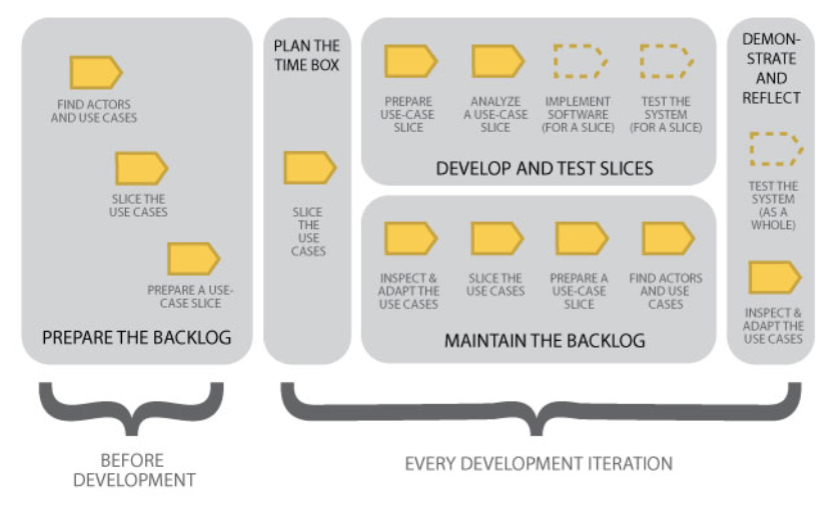
\includegraphics[width=0.8\textwidth]{figures/uc20_flow}
\caption{Use-case 2.0 activities for iterative development approaches}
\label{fig:usecase20:flow}
\end{figure}


\section{Involved Data}
\subsection{Actual data}
The data makes use of a small data set used to illustrate the use of survival analysis methodologies when teaching the subject. The data set is called ovarian and contains the survival in a randomised trial comparing two treatments for ovarian cancer. This has 26 cases and the following columns:
\begin{itemize}

\item futime: survival\footnote{Survival in days while not observing the event} or censoring time\footnote{Patient left the observation after this amount of time and the event didnt take place}
\item fustat: censoring status (1: survival, 0: censored\todo{Is this like this?})
\item age: of the patient in years
\item resid.ds: residual disease present (1=no,2=yes) 
\item rx: treatment group (integers)
\item ecog.ps: ECOG performance status (see \autoref{tab:ecog})
\end{itemize}

\subsection{Statistical Knowledge Base}
\begin{itemize}
	\item Models are suitable for research questions
	\item models have critical assumptions
	\item Models have non-critical assumptions (might be violated and can still be alright to use
	\item \texttt{m2 must fulfil the following critical assumptions ["a1", "a2"], ... }\insertref{Isabels follow up paper of example and data and models}
	\item \texttt{ Survival can be achieved by using the following model \{"m1"=>"a1", "m2"=>["a1", "a2"], "m3" =>["a1", "a3"]\}}
	\item Assumptions met given ($a_i$). Then we use AS1 ($m_i$ is a possible model if 
			\footnote{
				- Model $m_i$ achieves objective $o_c$\\
				- The data set meets the set of assumptions $A_t' = A_t (m_i)$\\
				- The research project meets the set of assumptions $A'_q = A_q (m_i)$\\
				- $A_c(m_i) \subseteq A_t' \cup A_q'$\\
				- $A_t$: Tests are assumptions that are assessed by applying a test on the available data set \\
				- $A_q$: queries are assumptions that are assessed by asking the clinician for an opinion.
			})
	\item R-Code (execution in Ruby possible \cite{rinRuby}  \insertref{https://github.com/clbustos/rinruby} \footnote{\texttt{rinruby} is a gem, that enables evaluation of R code in ruby}) and required outcomes for it decide, whether this model $m_i$ is possible or not. 
\end{itemize}
